\chapter{METHODOLOGY}
\thispagestyle{fancy}

    This chapter will present our newly developed deep reinforcement learning algorithm, called Adam-DQL, as well as going into some details regarding the implementation. This chapter will then disscuss about the software framework that is created to facilitate the research of this thesis. Alongside that, there will be some brief explanation about problems and quirks that may come with any implementation of a deep-reinforcement learning algorithm.
    
	\section{Adam-DQL Algorithm}
	\label{sec:4}
	\subsection{Problem Decomposition}
    	   
    Consider tasks in which an agent interacts with an environment,
    in this case the game itself, in a sequence of actions, observations and rewards.
    At each time-step the agent selects an action $a_t$ from the set of legal game actions,
    $A= { 1, . . ., K }$. The action is passed to the environment and modifies its internal state
    and the game score. In general the environment may be stochastic. The environment's
    internal state is not observed by the agent; instead the agent observes an image
    $x_t \in \mathbb{R}^d$ from the environment, which is a vector of pixel values representing the current screen. In addition it receives a reward $r_t$ representing the change in game score.
    Note that in general the game score may depend on the whole previous sequence of
    actions and observations; feedback about an action may only be received after many
    thousands of time-steps have elapsed.
    
    Because the agent only observes the current screen, the task is partially observed and many game states are perceptually aliased (that is, it is impossible to fully
    understand the current situation from only the current screen $x_t$ ). Therefore,
    sequences of actions and observations, $s_t= x_1 ,a_1 ,x_2 ,a_{t-1} ,x_t$ , are input to the
    algorithm, which then learns game strategies depending upon these sequences. All
    sequences in the environment are assumed to terminate in a finite number of time-
    steps. This formalism gives rise to a large but finite Markov decision process (MDP)
    in which each sequence is a distinct state, as explained in Section \ref{sec:21} As a result, one can apply standard reinforcement learning methods for MDPs that is already explained in \ref{sec:253}, simply by using the complete sequence $s_t$ as the state representation at time $t$.
	
	\subsection{Optimality for Value and Action}
	The goal of the agent is to interact with the environment by selecting actions in a way
    that maximizes future rewards. As shown in equation \ref{eq:23}, one can simply derive the Bellman optimality equation for $Q$, denoted as $Q^*(s,a)$, that is:
    
     \begin{equation}
            \begin{split}
                Q^*(s,a)& =\E(r_t+\gamma \max_{a'}Q^*(s_{t+1},a')|s_t=s,a_t=a) \\
                & = \sum_{s'}p(s'|s,a)[R(s,a,s')+\gamma\max_{a'}Q^*(s',a')]
            \end{split}
    \end{equation}
    
    The basic idea behind almost every reinforcement learning algorithm is to find a way to calculate the value of $Q^*$. This comes through iterative update, such that it converge to $Q*$, that is, $Q_i \to Q^*$ as $i \to \infty$. Here, Adam-DQL use the same basic update for temporal difference algorithm, that is:
    \begin{equation}
        Q_{i+1}(s,a)=\E[r+\gamma\max_{a'}Q_i^*(s',a')]
    \end{equation}
    
    However, as already explained in Section \ref{sec:253}, it is virtually impossible to compute that, especially since our algorithm is targeted towards complex game that has at least $100 \times 100$ pixels. Therefore, like \cite{mnih2015humanlevel}, we will also use deep neural networks to approximate the value of $Q^*$ function.
    
    \subsection{Adam-DQN}  
    For the sake of simplicity, our neural network that is used to approximate the $Q*$ will be called a Adam-DQN (Deep Q-network). The idea comes from the fact that mathematically, neural network is nothing more than a non-linear function. A simple modification to the $Q$-learning algorithm is made, by adding weights parameter $\theta$. Resulting in the same equation used by Deepmind's DQN \cite{mnih2015humanlevel}, that substitutes $r+\gamma\max_{a'}Q^*(s',a')$ with:
    
   \begin{equation}
      y=r+\gamma \max_{a'} Q(s',a';\theta_i^-)
   \end{equation}
    
	From here, Adam-DQN selects the \textbf{MSE} as the loss function, which resulted in the same equation as equation \ref{eq:36}
	
	    \begin{equation*}
             L(\theta_i)=\E_{s,a,r,s',i \sim D}[(r+\gamma \max_{a'}\hat{Q}(s',a',\theta_i^-)-Q(s,a,\theta_i))^2]
        \end{equation*}
    
    As with every optimization problem, to achieve optimality, we need to differentiate this loss function with the respect to weight/parameter $\theta$, which resulted in our final gradient approximation equation:
    
    \begin{equation}
            \nabla_{\theta_i}L(\theta_i)=\E_{s,a,r,s',i \sim D}[r+\gamma  \max_{a'}Q(s',a',\theta^-)-Q(s,a,\theta)\nabla_{\theta_i}Q_(s,a,\theta_i)]
    \end{equation}
    
    Now, the final task, is how to optimize(train) our neural network with our defined gradient, which will be discussed on the next section.
    
    \subsection{Training Algorithm for Adam-DQN}
    
    As indicated in section \ref{sec:342} the most common algorithm for training and optimizing is Stochastic Gradient Descent (SGD), it is also the algorithm of choice in \cite{DBLP:journals/corr/MnihKSGAWR13}. However, as the state space of the game grows larger and larger, using SGD might not be viable because of its main drawback, the convergence time. SGD has a tendency to either not reach the  global minima, because the speed of convergence (gradients) is too slow, or simply bounce back over and over without reaching convergence because the speed of convergence is too fast. RMSprop, an algorithm used by in \cite{mnih2015humanlevel}, is generally faster than SGD, because it uses 1st moments to accelerate or deccelerate the step towards convergence. However, as described in section \ref{sec:342}, RMSProp suffers from the fact that it has high bias early in the training because of the fact that it doesn't have a "correction" mechanism to prevent biases. This is the first major different of Adam-DQN compared to the Deepmind's original DQN \cite{DBLP:journals/corr/MnihKSGAWR13}. 
    \par
     Chapter \ref{sec:dql} already explained the need of deep neural networks to approximate the value of $Q(s,a)$. Adam-DQL uses Adam-DQN (Deep Q-Network), a deep convolutional neural network proposed by Deepmind to approximate the value of $Q(s,a)$. This section will discuss the computational process inside each operation in Deep Q-Network, which mainly consist of two parts, the forward pass (predicting the value of $Q(s,a)$) and the backward pass (training).
    \subsubsection{The Forward Pass - Prediction}
    The forward pass is the process of feeding the image from our game to our neural network, and receive the predicted $Q(s,a)$ values as an output. Deep Q-Network consists of 3 convolutional layers and 2 fully connected layers. 
    \begin{enumerate}
        \item \textbf{Convolutional Layers}
        This layer is what defined a convolutional neural networks. Convolutional layer \textit{interwine} two sources of information. Practically, convolutional layer builds a feature map that shows the likeability of a feature appearing in the image. This is achieved by applying a so called \textit{filter} or \textit{kernel} to an image. Filter is a matrix of weights analogous to a vector of weights in a standard feedforward neural network. The real values of the filter matrix change with each learning iteration over the training set, indicating that the network is learning to identify which regions are of significance for extracting features from the data. When applied to an image, denoted by operator $*$, small parts of the image matrix are taken (with the same size as the filter), and dot product of the image and the kernel is calculated. This will be the value of each entry in the feature maps. Below is an example of 1 filter applied to an $8 \times 8$ image matrix. 
        \begin{figure}[H]
        \centering
        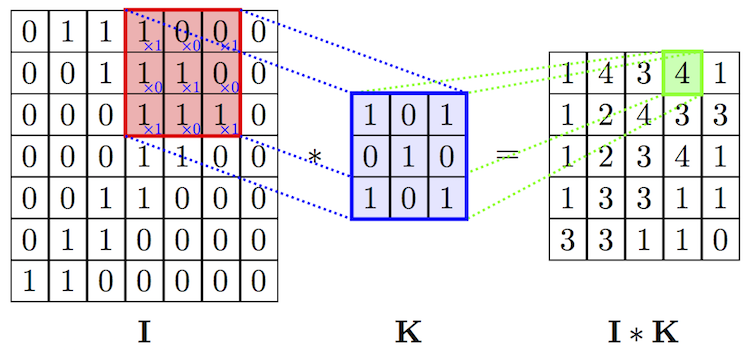
\includegraphics[scale=1.2]{images/convolve.png}
        \caption{Convolution applied to an 8 x 8 image}
        \label{fig:45}
        \end{figure}

        This patch (or \textit{window}) from the image is then slided by $m$ pixels, called stride, and then the filter is reapplied to get another element on the feature map. This process is repeated until all elements on the feature maps are filled. If the value of a specific element is big, it means that specific part of the image has a strong resemblance of the feature represented by the filter.
        \par
        Feature map is technically another image, which means another matrix. However, in this case it also reduces the size of the image while retaining the important information behind it. This operation is technically very similar to convolution operation in image and signal processing. However, in deep learning, instead of us (human) defining every values in the filter matrix, the value of filter matrix will be automatically adjusted (learned) by neural network, thus allowing neural network to find features by itself, hence the name deep convolutional neural network.  
        \par
        This operation is repeated for every convolutional layers. Since Adam-DQN has 3 convolutional layers, this operation will be applied 3 times and resulted in 64 feature maps of size $2 \times 2$. This feature maps will be fed to a  fully connected layer.
        \item \textbf{Fully Connected Layer}
        Fully connected layers are a simple feedforward neural network layers where each node is connected to every single node in the next layer. Fully connected layer utilizes the standard neural network operation, which is a linear combination (or dot product, in vector form) of all inputs and weights. The feature map from convolutional layer is flattened (from a matrix to a vector) and then the dot product of this vector and the weights vector is computed and then fed into the next fully connected layer. Since there are 64 feature maps with size $2 \times 2$, this layer has 256 ($64 \times 2 \times 2$) units/nodes/weights. This process is repeated for the last layer, resulting in a vector with 2-18 elements, depending on the game. Element $i$ in this vector represents the value of $Q^*(s,a_i)$. Which is our predicted $Q$ value for every action.
        \begin{figure}[H]
            \centering
            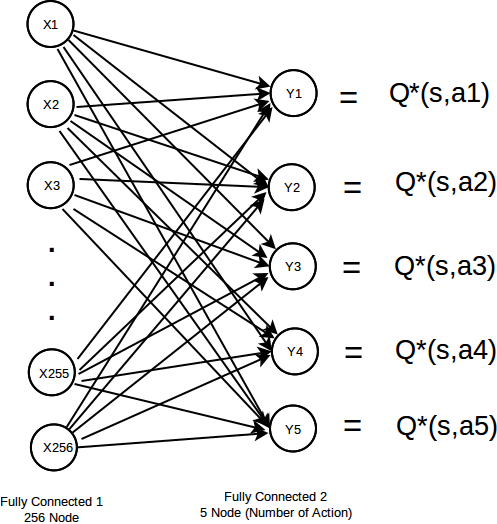
\includegraphics[scale=0.5]{images/FCLayer.png}
            \caption{Illustration of fully connected Layer operations}
            \label{fig:fclayer}
        \end{figure}
        Let the parameters (weights) for every unit in the first fully connected layer equals $\theta_{1 1},\theta_{1 2},\theta_{1 3}, ... , \theta_{256 \ 256} $, Then, the value of node $y_i$ in the next layer:
        \begin{align*}
            b_i&=x_1*\theta_{11}+x_2*\theta_{12}+x_3*\theta_{13}+...+x_{256}*\theta_{1 \ 256} \\
            y_i&=\phi(b_i)
        \end{align*}
        where $\phi()$ represents the activation function (in this case, ReLU). Then,as stated above, $y_i$ represents the value of $Q^*(s,a_i)$. From here, it is trivial to see which actions to take, which is simply $a^*=\argmax_a Q^*(s,a)$. 
        \end{enumerate}
        
        \subsubsection{The Backward Pass - Training}
        As with every other neural network, Deep Q-Network used in Adam-DQL also needs to be trained so that it creates accurate prediction. Adam-DQL uses the \textbf{MSE} (Mean squared error) since Adam-DQL is built to approximate $Q(s,a)$, which means this is a regression task. Similar to Deepmind's Deep Q-Learning, according to equation \ref{eq:36}, for a parameter $\theta_i$, the loss function would be:
        \begin{equation*}
            L(\theta_i)=\E_{s,a,r,s',i \sim D}[(r+\gamma \max_{a'}\hat{Q}(s',a',\theta_i^-)-Q(s,a,\theta_i))^2]
        \end{equation*}
        Where $(R(s,a)+\gamma \max_{a'}\hat{Q}(s',a',\theta_i^-)$ represents the target, and $Q(s,a,\theta_i)$ represents the current prediction. Therefore, given a state (an image of the game) at time $t$, denoted as $s_t$, the training process is as follows:
        \begin{enumerate}
            \item Do a forward pass with the state $s_t$ to the neural network, resulting in a vector $Y_t=[Q(s_t,a_1),Q(s_t,a_2),...]^T$ (see figure \ref{fig:fclayer}) which is the predicted $Q$-function.
            \item From the vector $Y_t$, select the best action $a^*_t$ where $Q(s_t,a^*_t)=\max_a Q(s_t,a)$, and perform that action in the game. The game should now return a new state $s_{t+1}$ as a reaction to $a^*_t$.
            \item Repeat the step 1-2 for $s_{t+1}$ , resulting in a new prediction $Y_{t+1}$ and best action $a^*_{t+1}$.
            \item Observe the reward $r_{t+1}$, and calculate $r_{t+1}+\gamma \max_{a'}\hat{Q}(s',a',\theta_i^-)$ where $\hat{Q}(s',a',\theta_i^-)$ simply means $Q(s_{t+1},a^*_{t+1})=\max_a Q(s_{t+1},a)$ (the maximum value of vector $Y_{t+1}$).
            \item Using the value from $Y_{t+1}$ and step 4, perform a backward pass and compute gradient for all parameters in the network.
        \end{enumerate}
        Using the same example as in figure \ref{fig:fclayer}, the backward pass for all the layers to compute the gradient is as follows:
        \begin{enumerate}
            \item \textbf{Fully Connected Layer} let $y^l_k$ denote the value of a node at layer $l$ and index $k$, from the forward pass:
            \begin{equation*}
                 y^{l+1}_k = \phi (y^l_1)\times \theta_{k1}+\phi (y^l_2) \times \theta_{k2}+\phi (y^l_3)\times \theta_{k3}+...+\phi (y^l_{256})\times \theta_{i256}
            \end{equation*}
            
            The gradient for a parameter $\theta_{ki}$ is then:
            \begin{equation*}
                \frac{\partial L(\theta_i)}{\partial \theta_{ki}}=\frac{\partial L(\theta_i)}{\partial y^{l+1}_k}\frac{\partial y^{l+1}_k}{\partial \theta{ki}}=\frac{\partial L(\theta_i)}{\partial y^{l+1}_k}\phi(y^l_i)
            \end{equation*}
           \item \textbf{Convolutional Layer} let $x^l_{kh}$ denote the value of an element in the layer $l$ and index $k,h$ in the filter.  
           \begin{figure}[H]
               \centering
               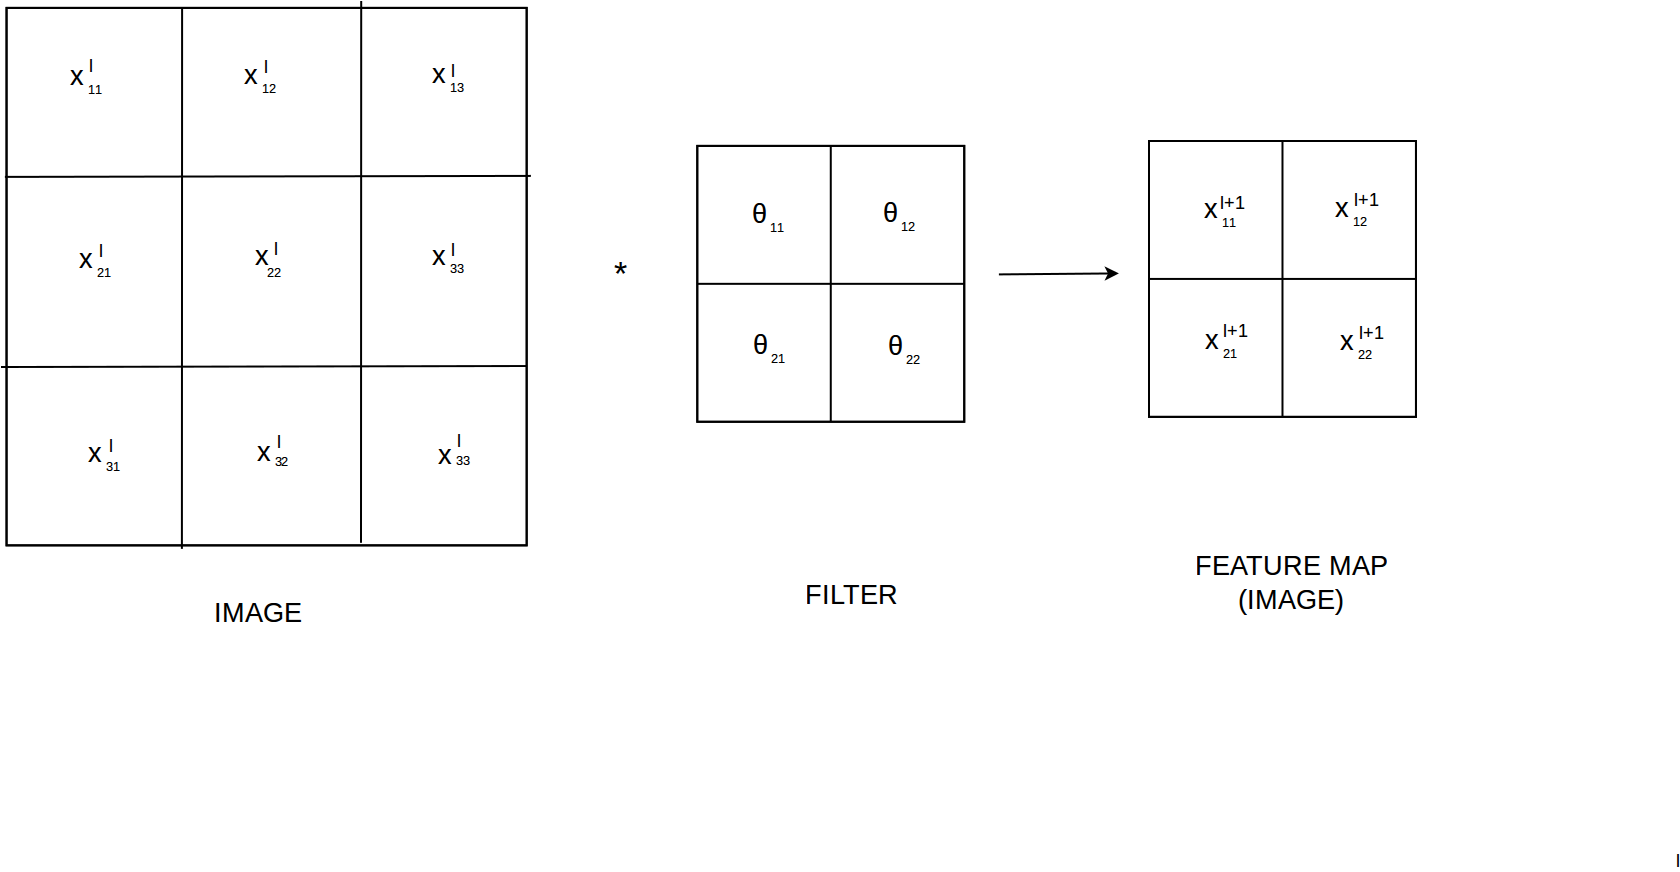
\includegraphics[scale=0.2]{images/convlayer2.png}
               \caption{Visualization of the convolutional layer operations}
               \label{fig:convlayer2}
           \end{figure}From the forward pass:
           \begin{equation*}
               y^{l+1}_{kh} = \phi (y^l_{kh})\times \theta_{11}+\phi (y^l_{k \ h+1}) \theta_{12}+\phi (y^l_{k+1 \ h}) \theta_{21} + \phi (y^l_{k+1 \ h+1}) \theta_{22}
           \end{equation*}
            The gradient for a parameter $\theta_{mn}$ is then:
           \begin{align*}
                \frac{\partial L(\theta_{mn})}{\partial \theta_{mn}}=& \frac{\partial L(\theta_{mn})}{\partial y^{l+1}_{kh}}\phi(y^l_{mn})+\frac{\partial L(\theta_{m \ n+1})}{\partial y^{l+1}_{m\ n+1}}\phi(y^l_{k \ h+1}) \\
                & +\frac{\partial L(\theta_{m+1 \ n})}{\partial y^{l+1}_{m+1\ n}}\phi(y^l_{k+1 \ h})+\frac{\partial L(\theta_{m +1\ n+1})}{\partial y^{l+1}_{m+1\ n+1}}\phi(y^l_{k+1 \ h+1})
            \end{align*}
        \end{enumerate}
    Now that the gradient for all layers can be computed, Adam optimization will be used to update the parameter, refer to section \ref{sec:342} for details.
    
    
    \subsection{Stability and Policy Improvement on Adam-DQN}
    
    As with every reinforcement learning problem, this method suffers from the same exploration-exploitation dilemma, where the agent has to choose whether to use current knowledge and move according to that, or try to explore more hoping that there may be some unexplored state-action combinations that will give us better result.
    \par
    To solve this problem, $\epsilon$-greedy algorithm will be used. As explained in Section \ref{section:26}, the agent will take a random action (exploration) with probability of $\epsilon$ and will take the best action according to current policy with probability $1 - \epsilon$.
    \par
    To further stabilize the Adam-DQN, stabilization technique that is proposed by Deepmind \cite{mnih2015humanlevel} , namely experience replay and target network freezing will be used.
    At each step of the training, dataset $D$ is sampled uniformly at random to get minibatch of experiences of size $M (( s, a, r, s' , i) \sim U (D))$ and perform learning (weights updates) on them.his approach has several advantages over standard online Q-learning. First, each step of experience
    is potentially used in many weight updates, which allows for greater data efficiency.
    Second, learning directly from consecutive samples is inefficient, owing to the strong
    correlations between the samples; randomizing the samples breaks these correlations and therefore reduces the variance of the updates. Third, when learning on-policy the current parameters determine the next data sample that the parameters are trained on. For example, if the maximizing action is to move left then the training samples will be dominated by samples from the left-hand side; if the maximizing action then switches to the right then the training distribution will also switch.
    \par
    It is easy to see how unwanted feedback loops may arise and the parameters could get
    stuck in a poor local minimum, or even diverge catastrophically. By using experience
    replay the behaviour distribution is averaged over many of its previous states,
    smoothing out learning and avoiding oscillations or divergence in the parameters.
    Note that when learning by experience replay, it is necessary to learn off-policy
    (because our current parameters are different to those used to generate the sample), which motivates the choice of Q-learning.
    \par
    The second modification to online $Q$-learning aimed at further improving the
    stability of our method with neural networks is to use a separate network for gen-
    erating the targets y j in the Q-learning update. More precisely, every C updates we
    clone the network $Q$ to obtain a target network $\hat{Q}$ and use $\hat{Q}$
    for generating the $Q$-learning targets y j for the following C updates to Q. This modification makes the
    algorithm more stable compared to standard online Q-learning, where an update
    that increases $Q(s_t ,a_t )$ often also increases $Q(s_{t_+1} ,a)$ for all $a$ and hence also increases
    the target $y_j$ , possibly leading to oscillations or divergence of the policy. Generating
    the targets using an older set of parameters adds a delay between the time an update
    to $Q$ is made and the time the update affects the targets $y_j$ , making divergence or oscillations much more unlikely.
    \par
    All stability improvement techniques explained above are already utilized by Deepmind in \cite{mnih2015humanlevel}. However, this thesis will present a new stability improvement techniques called \textbf{partial training}. On a case where the game $G$ can be broken into sub-problems $G_1, G_2, G_3, ...,G_k$ where $G_1$ represents the easiest sub-problem and $G_k$ represents the hardest sub-problem, our neural network $Q$ is trained for $G_1$ until satisfactory result is achieved. Then the neural network $Q$ is cloned and trained for $G_2$ until it also achieve satisfactory result. This process is repeated until the neural network $Q$ is trained for every sub-problem. Training the neural network on the easier sub-problem $G_1$ allows the neural network to get a lot of rewards (or punishment) allowing the training to proceed. On a case where the game is extremely hard, sometimes an agent might not be able to achieve any form of reward (or punishment), which prevents the actual training to proceed. By kickstarting the neural network on "simplified" version of the problem, our agent should get an idea about what it should do (or not do) on the current game environment faster.
    \par
    Lastly, this thesis will also add technique called \textbf{demonstration}. This technique is firstly utilized on reinforcement learning for robots \cite{DBLP:journals/corr/abs-1709-10089}. This thesis will utilize and use the idea for Adam-DQL to further kickstart the learning process, especially on a game with sparse rewards. On harder games where the rewards are really sparse, it's sometimes not possible for the random exploration (which happens in the early part of training process) to get a reward, thus preventing the neural network to learn and become better at the game. If the agent never gets better, it is very likely that the neural network will ended up diverging from the minima.
    \par
    Fortunately, it is possible to give neural network some initial "knowledge" \cite{DBLP:journals/corr/HesterVPLSPSDOA17} by feeding neural network some example of a proper transition $<s,a,r,s'>$. In layman terms, this means giving some basic state-action condition to built or learn upon. This will be achieved by storing human-created transitions $<s,a,r,s'>$ into the  replay memory $D$. This way, demonstration can be adapted into Adam-DQL as an initial step, without changing the flow of the algorithm itself. This human-created transition will then be replaced by actual replay memory from the agent, if the size replay memory buffer exceed the replay memory capacity.  
    
    \subsection{Preprocessing}
    \label{sec:preprocessing}
        The standard environment for modern games uses at least $256 \times 256$ pixels image for each frame. For modern technology, this is still considered low quality image. However, computing a multiple layers of convolutional neural network for this size is still very costly. Assuming only raw pixels are used, the convolutional part of the neural network needs to be on the same size. Not only convolutional layer that big is expensive both memory and CPU-wise, some part of the screen is mostly unused. Using that unused (unimportant) pixels as an input will only lead to divergence, since they adds more noise to our training data. Therefore, we need to define an preprocessing function $\phi$, that will crop the screen so that only the gameplay part of the screen is used. Preprocessing is a very vital process in Adam-DQL. Not only that it saves memory, it also further simplifies the features that the agent need to learn on the learning process. An image, in this case the game's screen capture, is represented as matrix of pixel values [0-255]. This thesis applies 2 preprocessing techniques, the first one is RGB to grayscale translation. For most games, colors don't actually contribute to how the game should be played, so it's logical to simply remove the colors and transform the image to grayscale. This is really important because it reduces the amount of matrices that will be fed to the neural network. Color image will have a 3 matrices associated with each image, one for each of the colour channels (red, green and blue). While grayscale image is simply a matrix of pixel values.
    \par
    The second one is image resizing, instead of using $256 \times 256$ pixels (the original image size), our processing map will resize the image to $84 \times 84$ pixels. This means our preprocessing map $\phi$ will output an $84 \times 84$ matrix with pixel values of [0-255]. 
    
    \begin{figure}[H]
        \centering
        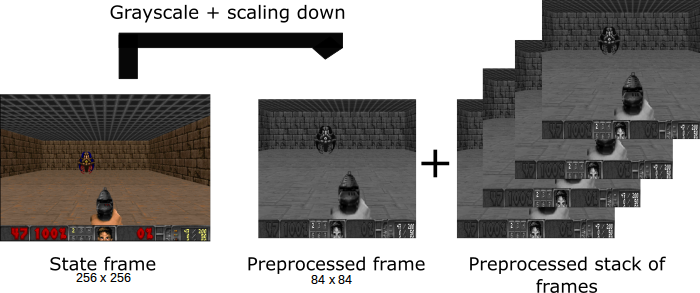
\includegraphics[scale=0.5]{images/preprocessing.png}
        \caption{Game Image Preprocessing}
        \label{fig:44}
    \end{figure}
    
    Also, 2-4 images will be used for every single step and stacked to each other, as 1 image simply cant represent any movement or condition. Which means our final output from this process is  $84 \times 84 \times 4$ (frame)  matrices.
    
    \subsection{Algorithm Review}

            \begin{algorithm}[H]\label{alg:7}
            
            \textbf{Require:} Replay memory $D$ with capacity $N$ \\
            \textbf{Require:} Initial parameter $\theta_0$ \\
            \textbf{Require:} Step size $\epsilon$ \\
            \textbf{Require:} Small constant $\delta $ for numerical stability \\
            \textbf{Require:} Exponential decay rate $\rho_1$ and $\rho_2$ \\
            \ForEach{episode $e$, unless stop condition satisfied}
                {
                
                Get initial state $s_0$ and preprocessed state $\phi_0$ \\
                Initialize 1st and 2nd moment variables $s=0, r=0$ \\
                Store demonstration data in replay memory $D$ \\
               \ForEach{timestep $t$ in current episode $e$}
                    {
                       Using $\epsilon$-greedy policy, select action $a_t$\\
                       Execute action $a_t$\\
                       Observe following state $s_{t+1}$ and and whether it is terminal ($i_{t+1}$)\\
                       Preprocess the state $\phi_{t+1}=\phi(s_{t+1})$ \\
                       Store transition $(\phi_{t},r_t,a_t,\phi_{t+1},i_{t+1})$\\
                       Sample random minibatch of transitions $(\phi_j,r_j,a_j,\phi_{j+1},i_{j+1})$   of size $M$ from $D$\\
                       \ForEach{sample in the minibatch}
                            {
                                \eIf{$i_j+1$ is true}{$y_j=r_j$}
                                {$y_j=r_j+\gamma \max_{a'}Q(\phi_{j+1},a',\theta)$}
                            }
                    }
                    Sample a minibatch of $m$ examples from the training set {$x^{(i)},...x^{(m)}$} and corresponding targets $y^{(i)}$ \\
                    Compute gradient estimate: $g \gets \frac{1}{m} \nabla_\theta \sum_i L(f(x^{(i)};\theta_e),y^{(i)}) $ \\
                    Update biased first and second moment estimate: $s,r \gets \rho_{1,2} (s,r)+ (1-\rho_{1,2})g$\\
                    Correct bias in first and second moment: $\hat{s},\hat{r} \gets \frac{s,r}{1-\rho_{1,2}^t}$\\
                    Compute update: $\Delta \theta_e \gets -\frac{\epsilon}{\delta+\sqrt{r}}\bigodot g.$ (Division and square root applied element-wise) \\
                    Apply update: $\theta_e \gets \theta_e +\Delta \theta_e$\\
                    
                }
                

            \caption{Adam-DQN with experience replay and demonstration}
            \end{algorithm}
    \section{Architecture}
    In order to show and experiment with the newly developed Adam-DQL, it is needed to create a software that allows experiment and testing on the new algorithm. Adam-DQL is specifically created to play more complex video-games, hence testing it by letting Adam-DQL agent to play video-games is a must. However, without a properly developed software, Adam-DQL is just program without any meaningful uses. Below is the details of the software developed for this thesis.
    \subsection{General Software Architecture}
    
    The software used in this thesis is shown on figure \ref{fig:41} and consists of 2 main components listed below. The reasoning behind this architechture is based on the analysis done in the next chapter. 
        \subsubsection{Games}
        This is the component that actually runs the game. Most of the time, the actual game source code is not available, Which means there's a need of some \textit{automated extraction} from the game, by utilizing modern desktop-PC features such as screenshot and screen capture, combined with the ability of the agent to simulate a key press on the keyboard. In the case where the game is open source, it's then possible to allow direct interactions between our agent and the game by simply modifying the game's source code. This thesis will provide an example for both cases, allowing the development of an AI that's as general as possible.
    
        \subsubsection{Deep Learning Agent}
        
        This is the \textit{brain} of the software framework. Coming from the fact that the code for all the game isn't available, and that the only accessible data is the pixels. It is needed to create a component to facilitate that so that our deep-learning agent (AI) will be able to interact with the game. This component will retrieve the pixel information from the game, \textit{preprocess} it, and send it to our actual agent in the program, as a preprocessed state ($\phi$).The agent can then process the data and  Whenever the agent decided to do something, the agent will send a signal to this component, that will simulate a button press, since this is the only input method acceptable by the game (unless source code of the game is available). Deep Learning agent will receive the input preprocessed by our framework, and use it as an input for Adam-DQL algorithm. After going through the neural network, Adam-DQL algorithm will send an output (as a signal) to the framework, then to the game. This process can happen in on the learning process (although the output might not be optimal yet) and the playing process (with optimal policy).
    
    \begin{figure}[H]
        \centering
        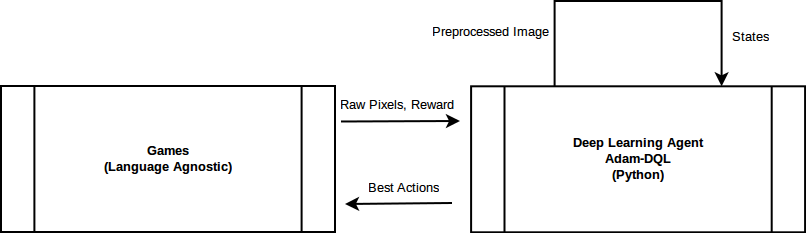
\includegraphics[scale=0.4]{images/framework2block.png}
        \caption{General software architecture}
        \label{fig:41}
    \end{figure}
    
    \subsection{State Representation}
        Despite the algorithm being applicable to a raw pixels as an input, simply putting all the raw pixels into the neural network is never a good idea. Technically, raw pixels contains all the information, that sometimes shouldn't be available for the players, for example: an agent shouldn't know that there's enemy 3 frames after the current frame. That's why Adam-DQN has a CNN (Convolutional neural network) to classify value of the pixels and change that into useful information. This information is then called \textit{classified data}, that will be selectively given to the agent for training. 
        \noindent
        This state representation for Adam-DQN is presented in figure \ref{fig:42}
        \begin{figure}[H]
            \centering
            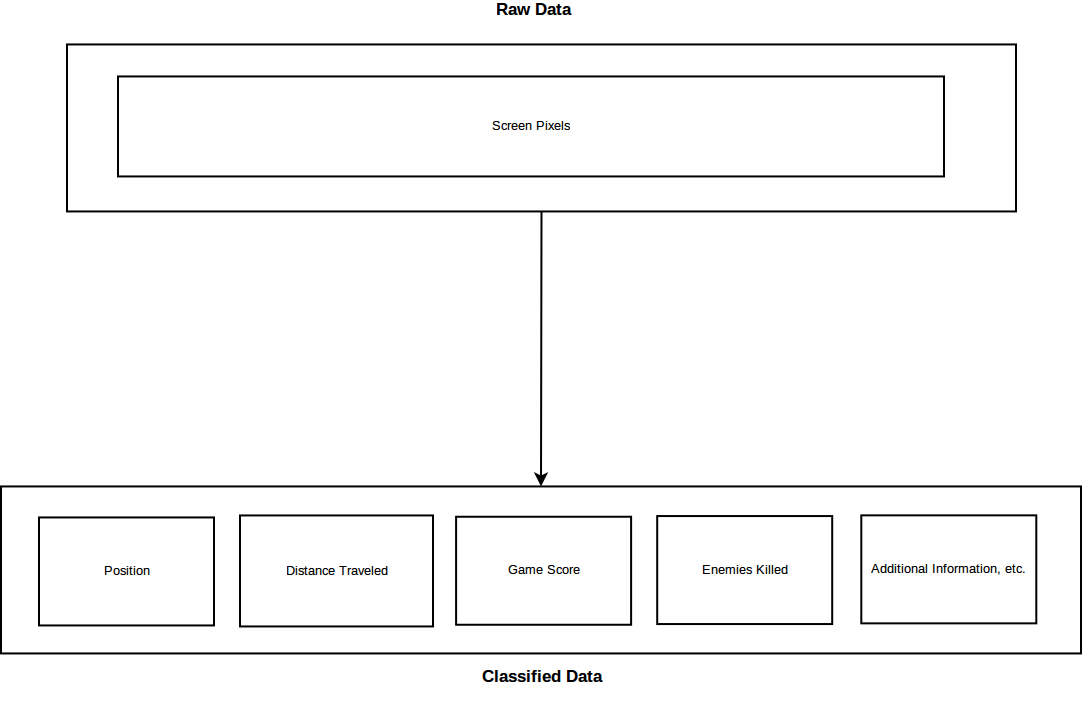
\includegraphics[scale=0.35]{images/data.png}
            \caption{State Representation Sample}
            \label{fig:42}
        \end{figure}
    
    
    \subsection{Neural Network Structure}
    The exact architecture of our neural network, shown schematically in figure 4.3, is as follows. The input to the neural network consists of an $84 \times 84 \times 4$ image produced by the preprocessing map $\phi$. The first hidden layer convolves 16 filters of $8\times 8$ with stride 4 with the input image and applies a rectifier nonlinearity. The second hidden layer convolves 32 filters of $4 \times 4$ with stride 2, again followed by a rectifier nonlinearity. This is followed by a third convolutional layer that convolves 64 filters of $2 \times 2$ with stride 1 followed by a rectifier. The final hidden layer is fully-connected and consists of 256 rectifier units. The output layer is a fully-connected linear layer with a single output for each valid action. The number of valid actions are generally around 2-18, depending on the game.
    
    \begin{figure}[H]
        \centering
        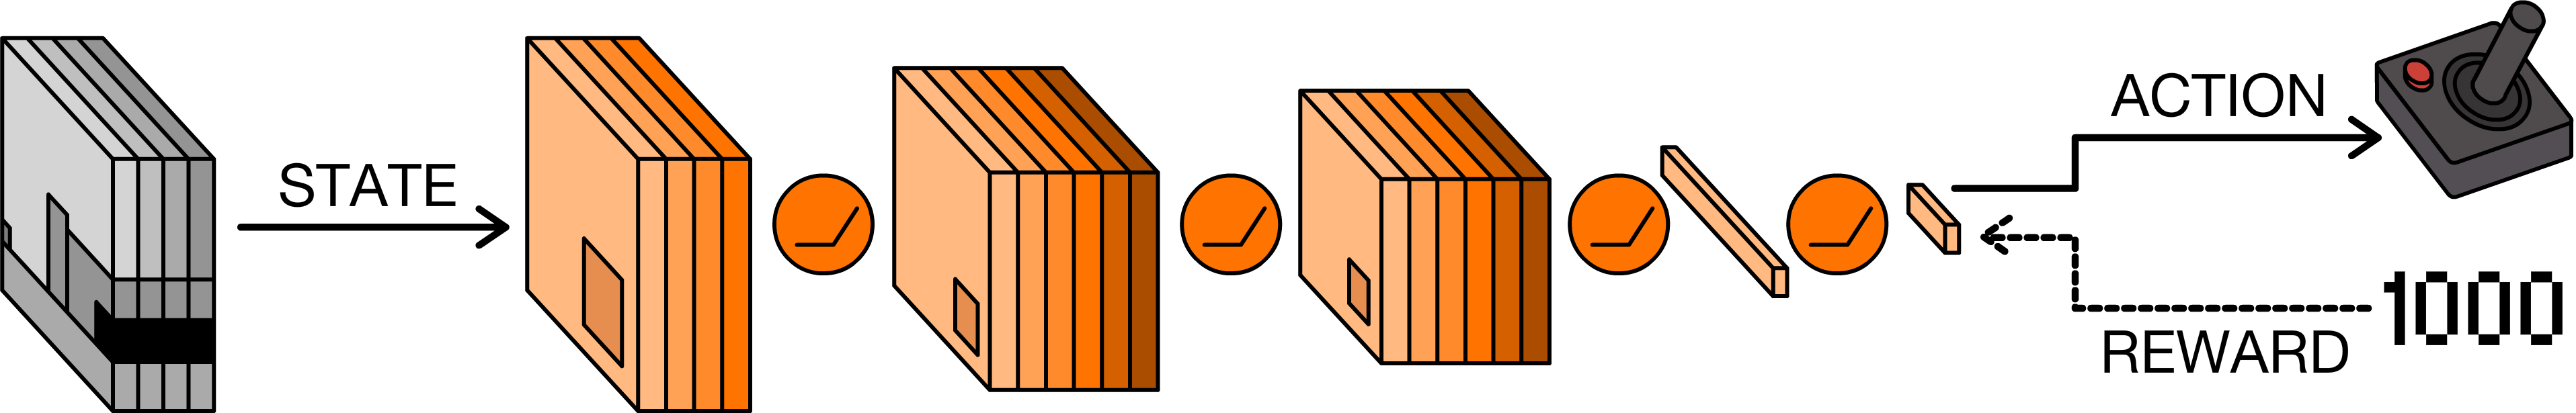
\includegraphics[scale=0.1]{images/dqn.png}
        \caption{Architecture of Adam-DQN}
        \label{fig:43}
    \end{figure}
    
    \iffalse
    \section{Implementation and Agent's Flow}
    In section \ref{sec:4}, Adam-DQL algorithm and its policy improvement strategy are explained. However, one might need additional explanation regarding how this algorithm should be implemented (programmatically). Therefore, this section is dedicated to explain the low level (program level) implementation of Adam-DQL algorithm. Adam-DQL requires states (pixels) and rewards to properly decide which action is optimal for a specific state. Thus, the process of getting an image until the decision of which actions to make will be explained in the following section.
    
    \subsection{Preprocessing}
    
    As stated in Section \ref{sec:preprocessing}, preprocessing is a very vital process in Adam-DQL. Not only that it saves memory, it also further simplifies the features that the agent need to learn on the learning process. An image, in this case the game's screen capture, is represented as matrix of pixel values [0-255]. This thesis applies 2 preprocessing techniques, the first one is RGB to grayscale translation. For most games, colors don't actually contribute to how the game should be played, so it's logical to simply remove the colors and transform the image to grayscale. This is really important because it reduces the amount of matrices that will be fed to the neural network. Color image will have a 3 matrices associated with each image, one for each of the colour channels (red, green and blue). While grayscale image is simply a matrix of pixel values.
    \par
    The second one is image resizing, instead of using $256 \times 256$ pixels (the original image size), our processing map will resize the image to $84 \times 84$ pixels. This means our preprocessing map $\phi$ will output an $84 \times 84$ matrix with pixel values of [0-255]. 
    
    \begin{figure}[H]
        \centering
        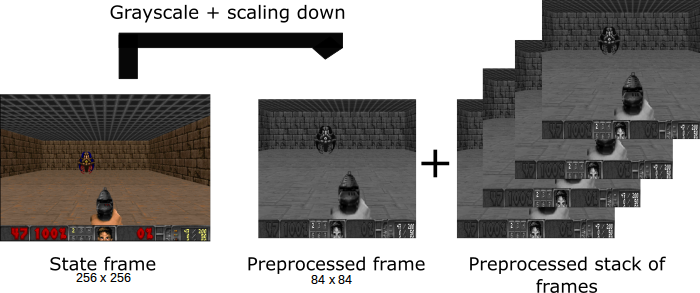
\includegraphics[scale=0.5]{images/preprocessing.png}
        \caption{Game Image Preprocessing}
        \label{fig:44}
    \end{figure}
    
    Also, as explained before, 4 images will be used for every single step and stacked to each other, as 1 image simply cant represent any movement or condition. Which means our final output from this process is  $84 \times 84 \times 4$ (frame)  matrices.
        
    \subsection{Deep Learning}
    Chapter \ref{sec:dql} already explained the need of deep neural networks to approximate the value of $Q(s,a)$. Adam-DQL uses DQN (Deep Q-Network), a deep convolutional neural network proposed by Deepmind to approximate the value of $Q(s,a)$. This section will discuss the computational process inside each operation in Deep Q-Network, which mainly consist of two parts, the forward pass (predicting the value of $Q(s,a)$) and the backward pass (training).
    \subsubsection{The Forward Pass - Prediction}
    The forward pass is the process of feeding the image from our game to our neural network, and receive the predicted $Q(s,a)$ values as an output. Deep Q-Network consists of 3 convolutional layers and 2 fully connected layers. 
    \begin{enumerate}
        \item \textbf{Convolutional Layers}
        This layer is what defined a convolutional neural networks. Convolutional layer \textit{interwine} two sources of information. Practically, convolutional layer builds a feature map that shows the likeability of a feature appearing in the image. This is achieved by applying a so called \textit{filter} or \textit{kernel} to an image. Filter is a matrix of weights analogous to a vector of weights in a standard feedforward neural network. The real values of the filter matrix change with each learning iteration over the training set, indicating that the network is learning to identify which regions are of significance for extracting features from the data. When applied to an image, denoted by operator $*$, small parts of the image matrix are taken (with the same size as the filter), and dot product of the image and the kernel is calculated. This will be the value of each entry in the feature maps. Below is an example of 1 filter applied to an $8 \times 8$ image matrix. 
        \begin{figure}[H]
        \centering
        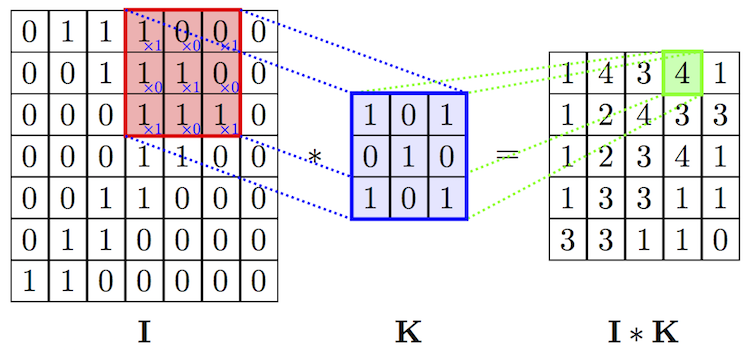
\includegraphics[scale=1.2]{images/convolve.png}
        \caption{Convolution applied to an 8 x 8 image}
        \label{fig:45}
        \end{figure}
        

        This patch (or \textit{window}) from the image is then slided by $m$ pixels, called stride, and then the filter is reapplied to get another element on the feature map. This process is repeated until all elements on the feature maps are filled. If the value of a specific element is big, it means that specific part of the image has a strong resemblance of the feature represented by the filter.
        \par
        Feature map is technically another image, which means another matrix. However, in this case it also reduces the size of the image while retaining the important information behind it. This operation is technically very similar to convolution operation in image and signal processing. However, in deep learning, instead of us (human) defining every values in the filter matrix, the value of filter matrix will be automatically adjusted (learned) by neural network, thus allowing neural network to find features by itself, hence the name deep convolutional neural network.  
        \par
        This operation is repeated for every convolutional layers. Since Adam-DQN has 3 convolutional layers, this operation will be applied 3 times and resulted in 64 feature maps of size $2 \times 2$. This feature maps will be fed to a  fully connected layer.
        \item \textbf{Fully Connected Layer}
        Fully connected layers are a simple feedforward neural network layers where each node is connected to every single node in the next layer. Fully connected layer utilizes the standard neural network operation, which is a linear combination (or dot product, in vector form) of all inputs and weights. The feature map from convolutional layer is flattened (from a matrix to a vector) and then the dot product of this vector and the weights vector is computed and then fed into the next fully connected layer. Since there are 64 feature maps with size $2 \times 2$, this layer has 256 ($64 \times 2 \times 2$) units/nodes/weights. This process is repeated for the last layer, resulting in a vector with 2-18 elements, depending on the game. Element $i$ in this vector represents the value of $Q^*(s,a_i)$. Which is our predicted $Q$ value for every action.
        \begin{figure}[H]
            \centering
            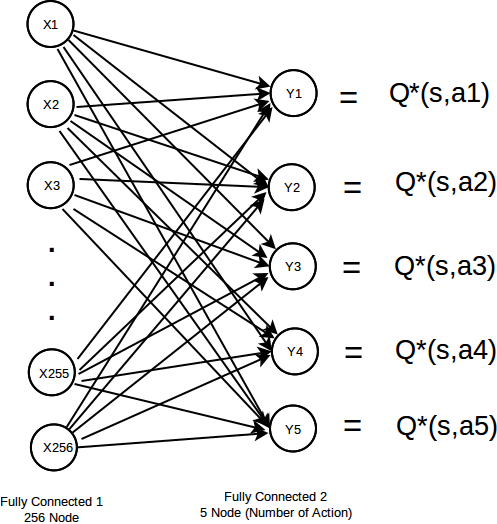
\includegraphics[scale=0.5]{images/FCLayer.png}
            \caption{Illustration of fully connected Layer calculations}
            \label{fig:fclayer}
        \end{figure}
        Let the parameters (weights) for every unit in the first fully connected layer equals $\theta_{1 1},\theta_{1 2},\theta_{1 3}, ... , \theta_{256 \ 256} $, Then, the value of node $y_i$ in the next layer:
        \begin{align*}
            b_i&=x_1*\theta_{11}+x_2*\theta_{12}+x_3*\theta_{13}+...+x_{256}*\theta_{1 \ 256} \\
            y_i&=\phi(b_i)
        \end{align*}
        where $\phi()$ represents the activation function (in this case, ReLU). Then,as stated above, $y_i$ represents the value of $Q^*(s,a_i)$. From here, it is trivial to see which actions to take, which is simply $a^*=\argmax_a Q^*(s,a)$. 
        \end{enumerate}
        
        \subsubsection{The Backward Pass - Training}
        As with every other neural network, Deep Q-Network used in Adam-DQL also needs to be trained so that it creates accurate prediction. Adam-DQL uses the \textbf{MSE} (Mean squared error) since Adam-DQL is built to approximate $Q(s,a)$, which means this is a regression task. Similar to Deepmind's Deep Q-Learning, according to Equation \ref{eq:36}, for a parameter $\theta_i$, the loss function would be:
        \begin{equation*}
            L(\theta_i)=\E_{s,a,r,s',i \sim D}[(r+\gamma \max_{a'}\hat{Q}(s',a',\theta_i^-)-Q(s,a,\theta_i))^2]
        \end{equation*}
        Where $(R(s,a)+\gamma \max_{a'}\hat{Q}(s',a',\theta_i^-)$ represents the target, and $Q(s,a,\theta_i)$ represents the current prediction. Therefore, given a state (an image of the game) at time $t$, denoted as $s_t$, the training process is as follows:
        \begin{enumerate}
            \item Do a forward pass with the state $s_t$ to the neural network, resulting in a vector $Y_t=[Q(s_t,a_1),Q(s_t,a_2),...]^T$ (see Figure \ref{fig:fclayer}) which is the predicted $Q$-function.
            \item From the vector $Y_t$, select the best action $a^*_t$ where $Q(s_t,a^*_t)=\max_a Q(s_t,a)$, and perform that action in the game. The game should now return a new state $s_{t+1}$ as a reaction to $a^*_t$.
            \item Repeat the step 1-2 for $s_{t+1}$ , resulting in a new prediction $Y_{t+1}$ and best action $a^*_{t+1}$.
            \item Observe the reward $r_{t+1}$, and calculate $r_{t+1}+\gamma \max_{a'}\hat{Q}(s',a',\theta_i^-)$ where $\hat{Q}(s',a',\theta_i^-)$ simply means $Q(s_{t+1},a^*_{t+1})=\max_a Q(s_{t+1},a)$ (the maximum value of vector $Y_{t+1}$).
            \item Using the value from $Y_{t+1}$ and step 4, perform a backward pass and compute gradient for all parameters in the network.
        \end{enumerate}
        Using the same example as in Figure \ref{fig:fclayer}, the backward pass for all the layers to compute the gradient is as follows:
        \begin{enumerate}
            \item \textbf{Fully Connected Layer} let $y^l_k$ denote the value of a node at layer $l$ and index $k$, from the forward pass:
            \begin{equation*}
                 y^{l+1}_k = \phi (y^l_1)\times \theta_{k1}+\phi (y^l_2) \times \theta_{k2}+\phi (y^l_3)\times \theta_{k3}+...+\phi (y^l_{256})\times \theta_{i256}
            \end{equation*}
            
            The gradient for a parameter $\theta_{ki}$ is then:
            \begin{equation*}
                \frac{\partial L(\theta_i)}{\partial \theta_{ki}}=\frac{\partial L(\theta_i)}{\partial y^{l+1}_k}\frac{\partial y^{l+1}_k}{\partial \theta{ki}}=\frac{\partial L(\theta_i)}{\partial y^{l+1}_k}\phi(y^l_i)
            \end{equation*}
           \item \textbf{Convolutional Layer} let $x^l_{kh}$ denote the value of an element in the layer $l$ and index $k,h$ in the filter.  
           \begin{figure}[H]
               \centering
               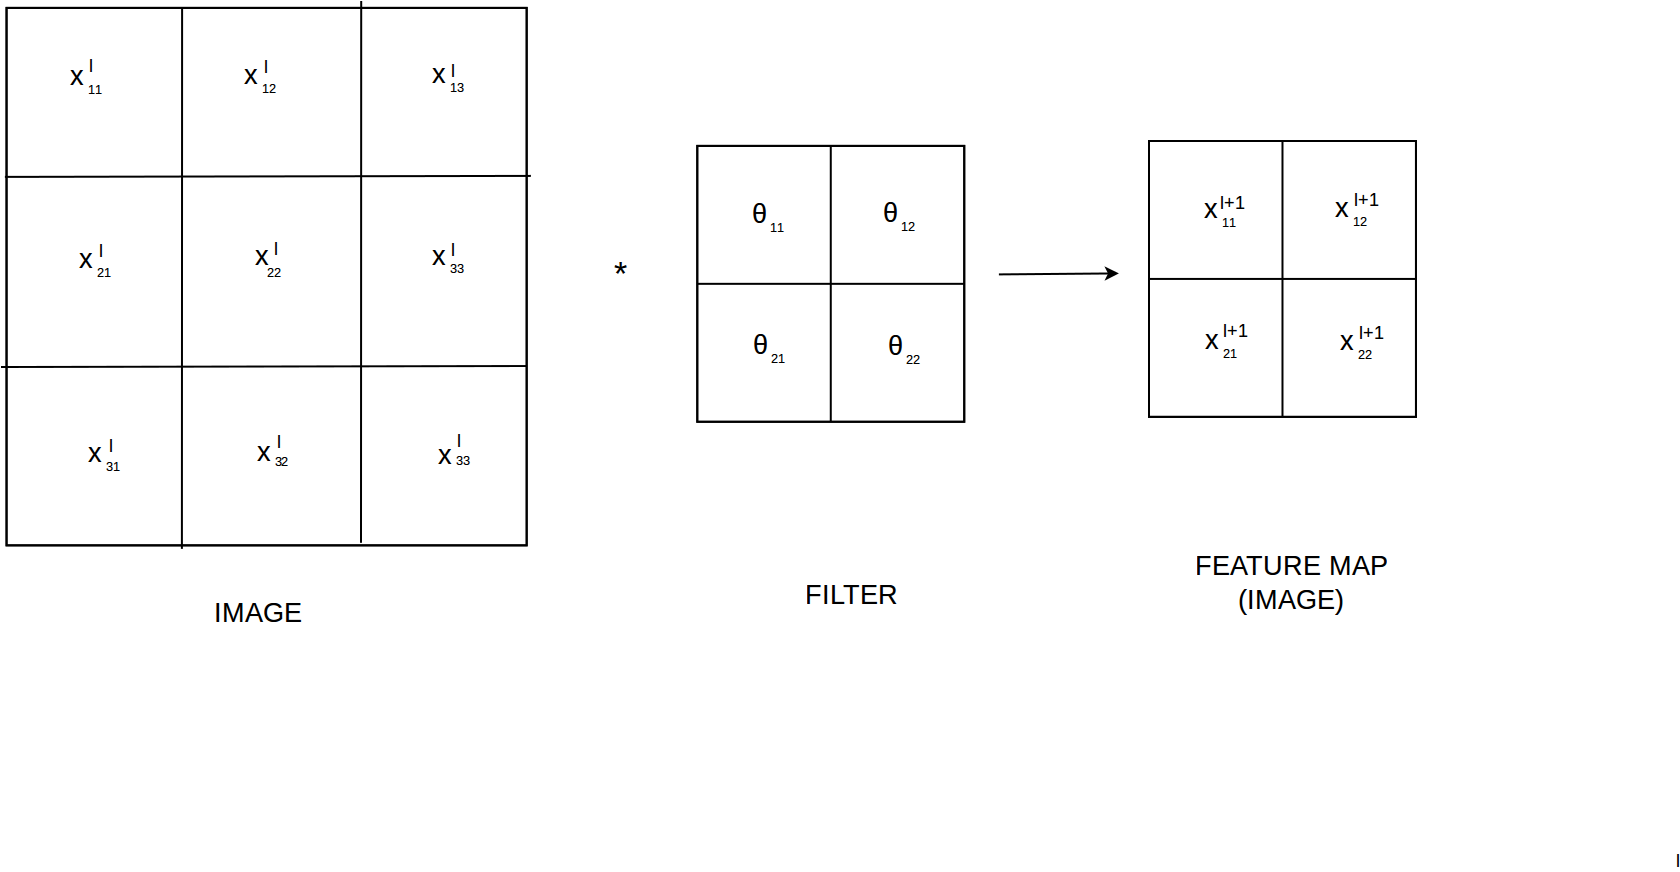
\includegraphics[scale=0.2]{images/convlayer2.png}
               \caption{Visualization of the convolutional layer operations}
               \label{fig:convlayer2}
           \end{figure}From the forward pass:
           \begin{equation*}
               y^{l+1}_{kh} = \phi (y^l_{kh})\times \theta{11}+\phi (y^l_{k \ h+1}) \theta{12}+\phi (y^l_{k+1 \ h}) \theta{21} + \phi (y^l_{k+1 \ h+1}) \theta{22}
           \end{equation*}
            The gradient for a parameter $\theta_{mn}$ is then:
           \begin{align*}
                \frac{\partial L(\theta_{mn})}{\partial \theta_{mn}}=& \frac{\partial L(\theta_{mn})}{\partial y^{l+1}_{kh}}\phi(y^l_{mn})+\frac{\partial L(\theta_{m \ n+1})}{\partial y^{l+1}_{m\ n+1}}\phi(y^l_{k \ h+1}) \\
                & +\frac{\partial L(\theta_{m+1 \ n})}{\partial y^{l+1}_{m+1\ n}}\phi(y^l_{k+1 \ h})+\frac{\partial L(\theta_{m +1\ n+1})}{\partial y^{l+1}_{m+1\ n+1}}\phi(y^l_{k+1 \ h+1})
            \end{align*}
        \end{enumerate}
    Now that the gradient for all layers can be computed, Adam optimization will be used to update the parameter, refer to Section \ref{sec:342} for details.
    \fi